
\section{Introduction}

\subsection{About InsightCAE}

InsightCAE is a workbench for Computer-Aided Engineering. Individual open source projects often meet only subtasks in analysis process. To automate repetitive computational tasks, a combination of several open source engineering software tools is often required. In order to use open source software productive and efficient for everyday tasks, the analysis automation framework InsightCAE was created.

InsightCAE serves as a framework for the implementation of analysis procedures. The objective is to provide interfaces to the tools and simulation programs that are needed for a specific computing task.

\subsection{License and Copyright}

This program is free software; you can redistribute it and/or modify it under the terms of version 2 of the GNU General Public License\footnote{\url{http://www.gnu.org/licenses/old-licenses/gpl-2.0.html}} as published by the Free Software Foundation. You accept the terms of this license by distributing or using this software.

This manual is Copyright (c) 2017 silentdynamics GmbH.

Permission is granted to copy, distribute and/or modify this document under the terms of the GNU Free Documentation License, Version 1.3 or any later version published by the Free Software Foundation; with no Invariant Sections, no Front-Cover Texts, and no Back-Cover Texts. A copy of the license is included in the section entitled "GNU Free Documentation License".

\subsection{Features and Highlights}

InsightCAE's objective is to create automated analysis workflows.
The high level API resides in the core "toolkit" library.
Automated workflows usually involve different external programs and utilities.
For the realization of automated workflows, it is sometimes required, to create add-ons to these external programs.
Thus InsightCAE is also a container for add-ons to other programs.

\begin{itemize}
\item InsightCAD script-based, fully parametric CAD

\begin{itemize}
    \item OpenCASCADE geometry kernel
    \item assemblies, constraint-based sketches, part library, drawing export
\end{itemize}

\item OpenFOAM add-ons (schemes, boundary conditions, models, ...)
\item Pre- \& Postprocessing tool (OpenFOAM Case Builder)
\item analysis workflow automation tools (GUI)
\end{itemize}



\subsection{Recommendations for Working with Shell-based Tools in Linux}

Sometimes it is necessary to execute tools in a bash shell, e.g. because no GUI for it is available. And often it is easier to keep an overview in graphical file manager.
Having a console window open together with a file manager window at the same time is an obvious solution but to do so for many cases at a time may easily confuse the desktop. 

Here are two useful hints to solve this issue:
 
\begin{enumerate}

 \item The KDE file manager \textbf{dolphin} offers the possibility to display a console in the lower half of the window. The working directory is synchronized with the directory shown in the graphical window by injection of \textbf{cd} commands. Vice versa, when the working directory is changed in the shell, the graphical display is updated as well.
 
 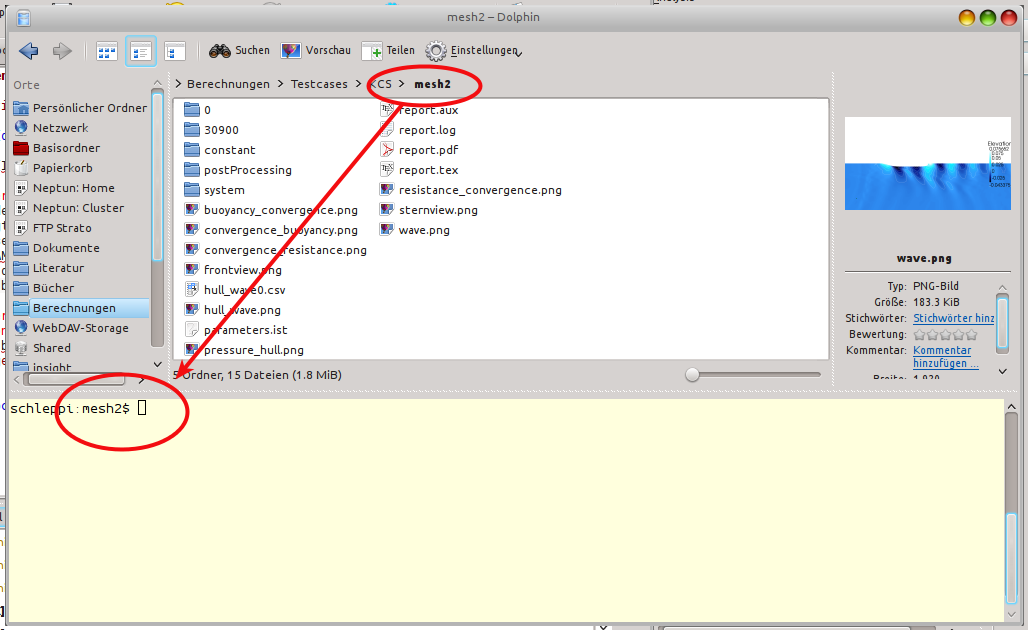
\includegraphics[width=\linewidth]{figs/intro/dolphin_with_terminal} 

 \item There is a Norton-Commander-like file manager named \textbf{krusader}. It offers the same functionality regarding the embedded terminal but a more flexible way of displaying multiple folders. In addition to the two list view on the left and right, multiple tabs for folders can be added in each list view. And there is also a rich interface to define custom commands and file associations.
 
 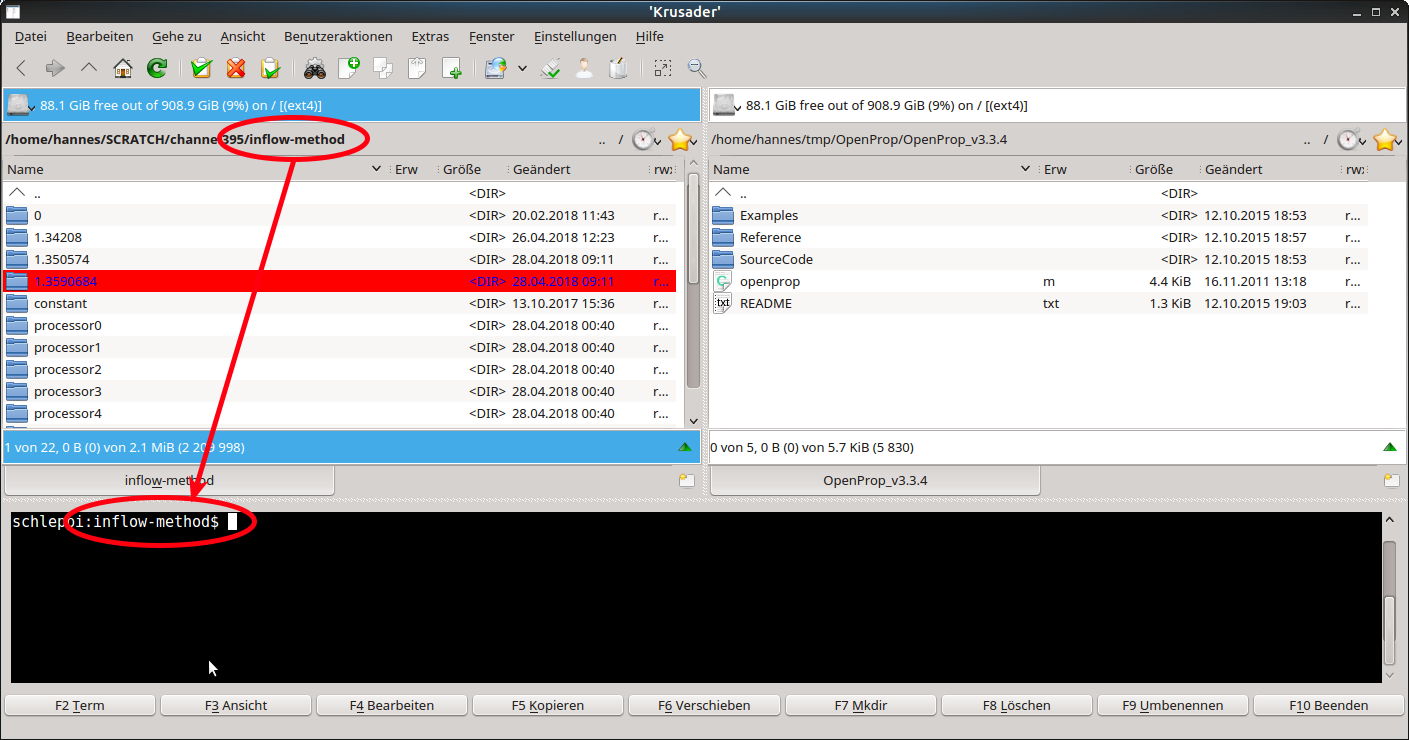
\includegraphics[width=\linewidth]{figs/intro/krusader_with_terminal}

\end{enumerate}


\subsection{Web Resources}

\begin{itemize}
\item Source Code Repository \url{https://github.com/hkroeger/insightcae}
\item Issue Tracker \url{https://github.com/hkroeger/insightcae/issues}
\item Web Forum \url{https://groups.google.com/forum/#!forum/insightcae}
\end{itemize}

\subsection{Reporting Bugs and Feature Requests}

Please use the issue tracker \url{https://github.com/hkroeger/insightcae/issues} to report any bugs.

We also monitor the web forum \url{https://groups.google.com/forum/#!forum/insightcae} for questions or feature requests.

\subsection{Getting Professional Help and Support}

Beyond the web resources above, silentdynamics GmbH offers commercial support\footnote{\url{http://silentdynamics.de/en/oss-cae/}} for professional users of InsightCAE. Automated analyses according to customer needs and specifications are implemented  by creating new specialized modules for Insight CAE.
Typical support contracts include also user training and continuous customization and updating of InsightCAE and its add-ons.